\documentclass[]{book}
\usepackage{lmodern}
\usepackage{amssymb,amsmath}
\usepackage{ifxetex,ifluatex}
\usepackage{fixltx2e} % provides \textsubscript
\ifnum 0\ifxetex 1\fi\ifluatex 1\fi=0 % if pdftex
  \usepackage[T1]{fontenc}
  \usepackage[utf8]{inputenc}
\else % if luatex or xelatex
  \ifxetex
    \usepackage{mathspec}
  \else
    \usepackage{fontspec}
  \fi
  \defaultfontfeatures{Ligatures=TeX,Scale=MatchLowercase}
\fi
% use upquote if available, for straight quotes in verbatim environments
\IfFileExists{upquote.sty}{\usepackage{upquote}}{}
% use microtype if available
\IfFileExists{microtype.sty}{%
\usepackage{microtype}
\UseMicrotypeSet[protrusion]{basicmath} % disable protrusion for tt fonts
}{}
\usepackage[margin=1in]{geometry}
\usepackage{hyperref}
\hypersetup{unicode=true,
            pdftitle={Estadística para el Análisis de Datos},
            pdfauthor={Gener Avilés R},
            pdfborder={0 0 0},
            breaklinks=true}
\urlstyle{same}  % don't use monospace font for urls
\usepackage{natbib}
\bibliographystyle{apalike}
\usepackage{longtable,booktabs}
\usepackage{graphicx,grffile}
\makeatletter
\def\maxwidth{\ifdim\Gin@nat@width>\linewidth\linewidth\else\Gin@nat@width\fi}
\def\maxheight{\ifdim\Gin@nat@height>\textheight\textheight\else\Gin@nat@height\fi}
\makeatother
% Scale images if necessary, so that they will not overflow the page
% margins by default, and it is still possible to overwrite the defaults
% using explicit options in \includegraphics[width, height, ...]{}
\setkeys{Gin}{width=\maxwidth,height=\maxheight,keepaspectratio}
\IfFileExists{parskip.sty}{%
\usepackage{parskip}
}{% else
\setlength{\parindent}{0pt}
\setlength{\parskip}{6pt plus 2pt minus 1pt}
}
\setlength{\emergencystretch}{3em}  % prevent overfull lines
\providecommand{\tightlist}{%
  \setlength{\itemsep}{0pt}\setlength{\parskip}{0pt}}
\setcounter{secnumdepth}{5}
% Redefines (sub)paragraphs to behave more like sections
\ifx\paragraph\undefined\else
\let\oldparagraph\paragraph
\renewcommand{\paragraph}[1]{\oldparagraph{#1}\mbox{}}
\fi
\ifx\subparagraph\undefined\else
\let\oldsubparagraph\subparagraph
\renewcommand{\subparagraph}[1]{\oldsubparagraph{#1}\mbox{}}
\fi

%%% Use protect on footnotes to avoid problems with footnotes in titles
\let\rmarkdownfootnote\footnote%
\def\footnote{\protect\rmarkdownfootnote}

%%% Change title format to be more compact
\usepackage{titling}

% Create subtitle command for use in maketitle
\newcommand{\subtitle}[1]{
  \posttitle{
    \begin{center}\large#1\end{center}
    }
}

\setlength{\droptitle}{-2em}
  \title{Estadística para el Análisis de Datos}
  \pretitle{\vspace{\droptitle}\centering\huge}
  \posttitle{\par}
  \author{Gener Avilés R}
  \preauthor{\centering\large\emph}
  \postauthor{\par}
  \predate{\centering\large\emph}
  \postdate{\par}
  \date{2017-02-19}

\usepackage{booktabs}
\usepackage{amsthm}
\makeatletter
\def\thm@space@setup{%
  \thm@preskip=8pt plus 2pt minus 4pt
  \thm@postskip=\thm@preskip
}
\makeatother

\begin{document}
\maketitle

{
\setcounter{tocdepth}{1}
\tableofcontents
}
\chapter{Introducción}\label{introduccion}

\chapter{Conceptos Generales}\label{conceptos-generales}

\textbf{7 de Febrero 2017}

\begin{itemize}
\tightlist
\item
  Cuando se tiene un modelo conocido que se asemeja al conjunto de
  datos, se le llama \textbf{modelo parametrico}. P.ej:
\end{itemize}

\[\int_{a}^{b} f(x)dx\]

\begin{itemize}
\tightlist
\item
  La robustez del modelo la da el \textbf{coeficiente de correlacion}
  (\(R^2\)), el cual nos habla de que tanto se parece el modelo a los
  datos. los valores van de \(0-1\), un valor \(>0.9\) se considera
  adecuado.
\item
  Cunado los datos no se parecen a un modelo ya conocido, se utilizan
  los modelos \textbf{no parametricos}.
\end{itemize}

\section{Teoria de Conjuntos}\label{teoria-de-conjuntos}

\subsection{Definiciones}\label{definiciones}

\begin{itemize}
\tightlist
\item
  \textbf{Conjunto}: Una coleccion de elementos con caracteristicas que
  comparten entre ellos.
\end{itemize}

\[A=\text{{1,2,3,4}}\] \[B = \text{{numeros enteros positivos}}\]
\[ C = \text{{numeros enteros > 3}} = \text{{4,5,6...}}\] Todos estos
tipos de conjuntos se pueden convertir eventualmente en el
\textbf{espacio muestral}, por lo tanto la definicion del espacio
muestral es vital antes de iniciar procesos de anlalisis.

\begin{itemize}
\tightlist
\item
  Alternativamente, los elementos \(x\) de un conjunto se pueden
  enunciar de tal manera que cumplan una caracteristica \(P\).
\end{itemize}

\[\text{{x|x satisface P}}\]

En esta notacion, el simbolo \emph{\(|\)} se interpreta como:
\textbf{\emph{``tal que''}}.

Otro ejemplo con esta notacion:

\[ E = \{x|x \space numero\space entero\space 4 \leq x \leq 10\}\]

\begin{itemize}
\tightlist
\item
  \textbf{Pertenece a (\(\in\)):}
\end{itemize}

Tomando el ejemplo anterior, podemos decir que \(x = 5 \in E\).

\begin{itemize}
\tightlist
\item
  \textbf{No pertenece a (\(\notin\))}
\end{itemize}

Tomando el ejemplo anterior podemos decir que \(x = 11 \notin E\)

\begin{itemize}
\tightlist
\item
  \textbf{Subconjunto (\(\subset\))}
\end{itemize}

Cuando todos los elementos del conjunto \(A\) estan incluidos en el
conjunto \(B\) (\(A \subset B\))

\begin{itemize}
\tightlist
\item
  \textbf{Complemento (\(^c\))}
\end{itemize}

El complemento de un conjunto \(S\), con respecto al conjunto universo
(\(\Omega\)), otros autores utilizan \(U\), es el conjunto de todos los
elementos que no pertenecen a \(S\), y se denota como \(S^c\). Es
importante recordar que \(\Omega^c = \emptyset\) donde \(\emptyset\) es
el conjunto vacio.

\begin{itemize}
\tightlist
\item
  \textbf{Union (\(\cup\))}
\end{itemize}

\[S \cup T = \{x|x \in or\space x\in T\}\]

\begin{itemize}
\tightlist
\item
  \textbf{Intereseccion (\(\cap\))}
\end{itemize}

\[S \cap T = \{x|x \in S\space y \space x \in T \} \]

 Por lo tanto:

\[\bigcup_{n=1}^{\infty}= S_1 \cup S_2 \cup ...= \{ x|x \in S_n para \space alguna\space n\} \]
Donde \(para\space S_n = \space un \space entero \space positivo\).

\[ \bigcap_{n=1}^{\infty} = S_1 \cap S_2 \cap ... = \{ x|x \in S_n \space para \space alguna \space n\}\]

\subsection{Conjuntos Disjuntos}\label{conjuntos-disjuntos}

\begin{itemize}
\tightlist
\item
  Son aquellos cuya interseccion (\(\cap\)) es el conjunto vacio
  (\(\emptyset\)).
\item
  No se intersectan.
\end{itemize}

\[S \cap T = \{ \emptyset\}\] La probabilidad del conjunto vacio no es
igual a \(\emptyset\), por lo tanto habra que calcularla en cada caso.

\subsection{Partición:}\label{particion}

Una colección de conjuntos se dice que es una particion de un conjunto
\(S\) si los conjuntos en la coleccion son disjuntos y su union es
\(S\).

\[S = \{1,2,3,4,5,6,7,8\}\] \(A = \{1,2,3\}\), \(B = \{4,5,6,7,8\}\) y
\(C = \{\emptyset\}\)

 \textbf{Ojo: simpre considerar la probabilidad del conjunto vacio,
siempre existe.}

\begin{itemize}
\tightlist
\item
  Si \(x\) y \(y\) son 2 objetos \((x,y)\) para describir un par
  ordenado, por ejemplo, numeros reales \(R\), el conjunto de pares (o
  tripleta) de escalares se puede escribir como \(R^2\) y \(R^3\),
  respectivamente.
\end{itemize}

\section{Diagramas de Venn}\label{diagramas-de-venn}

 \(A \cap B\)

\begin{figure}[htbp]
\centering
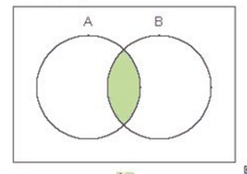
\includegraphics{D:/Dropbox/MsC UABC/2o Semestre/Clases/Estadistica/estadistica-syllabus/img/venn.png}
\caption{}
\end{figure}

\(A\cup B\)

\begin{figure}[htbp]
\centering
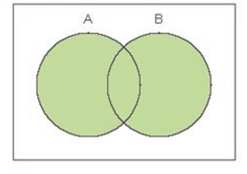
\includegraphics{D:/Dropbox/MsC UABC/2o Semestre/Clases/Estadistica/estadistica-syllabus/img/venn1.png}
\caption{}
\end{figure}

\(A^c \cap B\)

\begin{figure}[htbp]
\centering
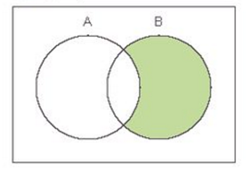
\includegraphics{D:/Dropbox/MsC UABC/2o Semestre/Clases/Estadistica/estadistica-syllabus/img/venn2.png}
\caption{}
\end{figure}

\(\text{Conjuntos Disjuntos}\)

\begin{figure}[htbp]
\centering
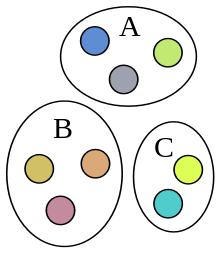
\includegraphics{D:/Dropbox/MsC UABC/2o Semestre/Clases/Estadistica/estadistica-syllabus/img/venn4.png}
\caption{}
\end{figure}

\(S,T,\space y \space V \space son \space una \space particion \space de \space \Omega\)

\begin{figure}[htbp]
\centering
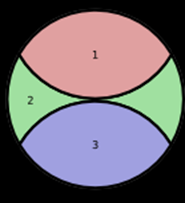
\includegraphics{D:/Dropbox/MsC UABC/2o Semestre/Clases/Estadistica/estadistica-syllabus/img/venn3.png}
\caption{}
\end{figure}

\section{Algebra de Conjuntos}\label{algebra-de-conjuntos}

\textbf{\emph{Propiedad asociativa ????}} \[S \cup T = T \cup S\]
\[S \cap (T \cup V) = (S \cap T) \cup (S \cap V)\] \[(S^c)^c = S\]
\[S \cup \Omega = \Omega\] \textbf{\emph{Propiedad Distributiva????}}

\[S \cup (T \cup V) = (S \cup T)\cup V\]
\[S \cup (T \cap V) = (S \cup T)\cap (S \cap V)\]
\[S \cap S^c = \emptyset\] \[S \cap \Omega = S\]

\section{Leyes de Morgan}\label{leyes-de-morgan}

Considerar las siguentes notaciones:
\((\bigcup_{n}^{}S_n)^c = \bigcap_{n}^{}{S_n}^c\)\\
 \((\bigcap S_n)^2 = \bigcup_{n}^{}{S_n}^c\)

*Notar como cambian de \(\cup\) a \(\cap\) y viceversa, en estas leyes.

\textbf{8 de Febrero de 2017}

\section{Modelos De Probabilidad}\label{modelos-de-probabilidad}

Buscan proveer certidumbre o reducir incertidumbre.

\subsection{Elementos de un Modelo de
Probabilidad}\label{elementos-de-un-modelo-de-probabilidad}

\begin{itemize}
\tightlist
\item
  El \textbf{espacio muestral (\(\Omega\))}: Entendido como el conjunto
  de todos los posibles resultados de un experimento.
\item
  \textbf{Ley de probabilidad}, la cual asigna a un conjunto \(A\) de
  posibles resultados (llamdo también evento) un número no-negativo
  (\(P(A) = (\text{la probabilidad de A})\)) que codifica nuestro
  conocimiento o creencia sobre la probabilidad de los elementos de
  \(A\).
\end{itemize}

\subsection{Axiomas de Probabilidad}\label{axiomas-de-probabilidad}

\begin{enumerate}
\def\labelenumi{\arabic{enumi}.}
\tightlist
\item
  \textbf{No negatividad} Para cada uno de los eventos en \(A\):
  \(P(A) \geq 0\)
\item
  \textbf{Adición} Si \(A\) y \(B\) son dos eventos disjuntos, entonces
  la posibilidad de su unión satisface: \(P(A \cup B) = P(A)+P(B)\)
  \textbf{ó} \(P(A_1\cup A_2 \cup ...A_n) = P(A_1) + P(A_2)+...P(A_n)\)
\item
  \textbf{Normalización} La probabilidad del copmleto (\emph{entire})
  espacio muestral \(\Omega\) es \(1\), esto es \(P(\Omega) = 1\).
\end{enumerate}

 \textbf{Ojo:} Los eventos del espacio muestral deben ser eventos
\textbf{\emph{mutuamente excluyentes}}, osea que no puedan suceder
simultaneamente.

\subsection{Ley de Probabilidad
Discreta}\label{ley-de-probabilidad-discreta}

\textbf{Probabilidad discreta:} Asignar a un evento una probabilidad
única (valor).

Si el espacio de probabilidad consiste de un número finito de posibles
resultados, entonces la ley de probabilidad se especifica por las
probabilidades de cada uno de los eventos. En particular, la
probabilidad de cualquier evento. \(\{S_1,S_2,...S_n\}\) es la suma de
las probabilidades de sus elementos:
\[P(\{S_1,S_2,...S_n\}) = P(S_1)+P(S_2)+...+P(S_n)\]

\subsection{Ley de Probabilidad Discreta
Uniforme}\label{ley-de-probabilidad-discreta-uniforme}

Si el espacio muestral consiste de \(n\) posibles resultados con igual
probabilidad de ocurrencia, entonces la probabilidad de cualquier evneto
\(A\), está dada por:
\[P(A)= \frac{\text{Número de elementos de A}}{n}\]

\subsection{\texorpdfstring{Función \emph{Densidad de
Probabilidad}}{Función Densidad de Probabilidad}}\label{funcion-densidad-de-probabilidad}

\begin{itemize}
\tightlist
\item
  También conocida como \emph{Probability Density Function (pdf)} o
  \emph{Probability Mass Function (pmf)}.
\end{itemize}

Para una variable aleatoria o evento discreto, se define como:
\[f(x) = P(X=x)\]

\subsection{\texorpdfstring{Acumulativa pdf (\emph{Comulative
pdf})}{Acumulativa pdf (Comulative pdf)}}\label{acumulativa-pdf-comulative-pdf}

\begin{itemize}
\tightlist
\item
  Se define como la suma de los resultados parcials de los eventos que
  validan el experimento:
\end{itemize}

\[cpdf = \sum_{i}(P(x_i=x))\]

Para los \(x_i\) que validan el experimento.

\textbf{14 de Febrero 2017}

\section{Probabilidad Condicional}\label{probabilidad-condicional}

La siguiente ecuación:

\[P(A/B) = \frac{P(A\cap B)}{P(B)}\]

Puede también ser expresada en los términos de \emph{probabilidad
condicional secuencial}: \[P(A\cap B) = P(A/B)*P(B)\] Siempre y cuando
\(P(B)>0\)

Si los posibles resultados tienen la misma probabilidad de ocurrencia
entonces:
\[P(A/B) = \frac{\text{No. de elementos en } A\cap B}{\text{No. de elementos en }B}\]

\textbf{Importante:} El conjunto universo en la probabilidad condicional
(dado un evento anterior) cambia de \(\Omega\) al subconjunto \(B\).

\subsubsection{Ejemplos:}\label{ejemplos}

\begin{itemize}
\tightlist
\item
  \textbf{Considerar el lanzamiento de 2 dados:}
\end{itemize}

\[A = \{\text{la suma es}\geq 8 \space y \space \leq 10\}\]
\[B = \{\text{el dado 1}=6 \} \therefore P(B) = \frac {1}{6}\]
Recordando los conceptos de combinaciones: \(C = n^m\) cuando \(n\) es
el número de posibles resultados y \(m\), el número de experimentos.
para éste ejemplo en particular las combinaciones posibles son
\(6^2 = 36\), entonces:
\[P(A\cap B) = \frac {3}{36} \therefore P(A/B) = \frac {\frac {3}{36}}{\frac {1}{6}} = \frac {18}{36} = \frac {1}{2}\]
Es importante que la probabilidad condicional es mayor a la probabilidad
independiente de previos eventos, porque el universo en la condicional
disminuye de \(\Omega\) a un subconjunto, en éste caso \(B\).

\begin{itemize}
\item
  \textbf{La probabilidad de que, al lanzar los dados del ejemplo
  anterior, la suma sea \(\geq 8\) y \(\leq 10\) ó
  \(A = \{\geq 8 \space y \space \leq 10\}.\)}

  A ésta probabilidad la denotaremos como \(P(A)\), al realizar el
  experimento manual obtenemos la siguiente imagen:

  \begin{figure}[htbp]
  \centering
  \includegraphics{D:/Dropbox/MsC UABC/2o Semestre/Clases/Estadistica/estadistica-syllabus/img/2017-02-14 11.40.56.jpg}
  \caption{}
  \end{figure}

   Se puede observar que se han indicado las combinaciones que cumplen
  con una suma \(\geq 8\) y \(\leq 10\) ó
  \(A = \{\geq 8 \space y \space \leq 10\}\).

  Por lo tanto: \[P(A) = \frac {12}{36} = \frac {1}{3}\].

  Otra manera de entender éste concepto es visualizarlo a través de una
  matriz:

  \begin{figure}[htbp]
  \centering
  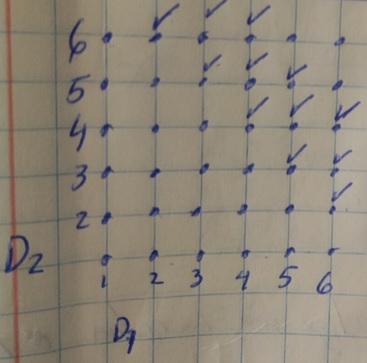
\includegraphics{D:/Dropbox/MsC UABC/2o Semestre/Clases/Estadistica/estadistica-syllabus/img/2017-02-14 12.56.55 mod.jpg}
  \caption{}
  \end{figure}
\end{itemize}

Con la visualización, es sencillo llegar a la conclusión
\(A = \frac {12}{36} = \frac {1}{3}\)

\begin{itemize}
\tightlist
\item
  \textbf{En el lanzamiento sucesivo de 3 monedas, queremos saber la
  probabilidad condicional, \(P(A/B)\), cuando \(A\) y \(B\) son los
  eventos:} \[A = \{\text{aparecen más soles que águilas}\}\]
  \[B = \{\text{el primer lanzamiento cae sol}\}\] La visualización de
  todas las posibilidades de éste fenómeno se puede apreciar en la
  siguiente figura:
\end{itemize}

\begin{figure}[htbp]
\centering
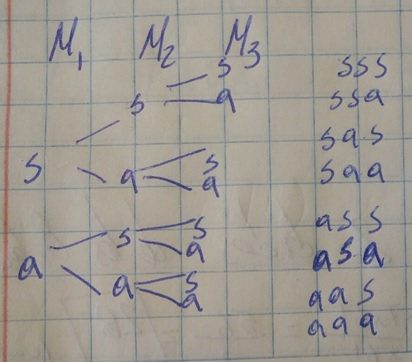
\includegraphics{D:/Dropbox/MsC UABC/2o Semestre/Clases/Estadistica/estadistica-syllabus/img/2017-02-14 12.57.08 mod.jpg}
\caption{}
\end{figure}

Derivado del árbol en la imagen se pueden determinar las probabilidades
de los siguientes subconjuntos:
\[P(A) = \{\text{sss, ssa, sas, ass }\} = \frac {4}{8} = \frac {1}{2}\]

\[P(B) = \{\text{sss, ssa, sas, saa}\} = \frac{4}{8} = \frac{1}{2}\]
\[P(A\cap B) = \{\text{sss, ssa, sas}\} = \frac{3}{8}\]

\[\therefore\]
\[P(A/B) = \frac {P(A\cap B)}{P(B)} = \frac {\frac {3}{8}}{\frac {1}{2}} = \frac {6}{8} = \frac {3}{4}\]
\textbf{\emph{Nótese el la mayor probabilidad de \(P(A/B)\) dado que el
universo pasó de ser \(\Omega\) al subconjunto \(B\).}}

\subsection{Repaso de combinaciones y
permutaciones}\label{repaso-de-combinaciones-y-permutaciones}

 La cantidad total de combinaciones posibles en un experimento se puede
calcular como \(n^m\) donde: \[n = \text{posibles resutlados}\]
\[m = \text{número de experimentos a realizar}\]

\begin{itemize}
\item
  Cuando de un número de combinaciones se elige una muestra \(r\) y el
  orden en el que éstas se elige no importa (\emph{combinaciones}):
  \[P = \left( \begin{array}{c} n \\ r \end{array} \right) = \frac {n!}{r!(n-r)!}\]
\item
  Cuando de un numero de combinaciones se elige una muestra \(r\) y el
  orden en el que ésta se elige \textbf{SI} importa
  (\emph{permutaciones}):
  \[P = \left( \begin{array}{c} n \\ r \end{array} \right) = \frac {n!}{(n-r)!}\]
\end{itemize}

\subsubsection{Ejemplo:}\label{ejemplo}

Al lanzar 8 dados, ¿cuántas combinaciones diferentes son posibles?
\[C = 6^8\] \textbf{PENDIENTE REVISAR}- Si elijo el resultado de 2 dados
de los 8 lanzados, ¿de cuántas maneras distintas los puedo elegir?:

\[P = \left( \begin{array}{c} 8 \\ 2 \end{array} \right) = \frac {n!}{r!(n-r)!}\]

Siempre y cuando \(A_1\) y \(A_2\) sean eventos disjuntos
(\(P(A_1\cap A_2) = \emptyset\)) podemos entonces decir que:

\[P = (A_1 \cap A_2 \vert B) = \frac {P(A_1 \cap B)}{P(B)}+ \frac {P(A_2 \cap B)}{P(B)} = P(A_1/B) + P(A_2/B)\]

\subsubsection{Ejemplo}\label{ejemplo-1}

Tomando datos del experimento anterior con monedas:

\[A_1 = \{\text{aparecen más soles que águilas}\} = \{\text{sss, ssa, sas, ass}\}\]
\[A_2 = \{\text{aparecen más águilas que soles}\} = \{\text{ssa, asa, aas, aaa}\}\]
\[B = \{\text{el primer lanzamiento es sol}\} = \{\text{sss, ssa, sas, saa}\}\]
\[A_1 \cap A_2 = \{\emptyset\}\] \[\therefore\]
\[P(A_1) = \frac {4}{8} = \frac {1}{4}\space \& \space P(A_2) = \frac {4}{8} = \frac {1}{4}\]
\[P(A_1\cap B) = \frac{3}{8}\] \[P(A_2\cap B) = \frac{1}{8}\]
\[P(A_1\cup A_2\vert B) = \frac {\frac{3}{8}}{\frac{1}{2}} + \frac{\frac{1}{8}}{\frac{1}{2}} = \frac{6}{8} + \frac{2}{8} = 1\]
\[P(A_1\cup A_2\vert B) = 1 \space \therefore\]
\[P(A_1\cup A_2...\cup A_i \vert B) = P(A_1/B) + P(A_2/B)+...+ P(A_i/B)\]
Siempre y cuando \(\{A_1\cap A_2...\cap A_i\}= \emptyset\).

\subsection{Independencia}\label{independencia}

Si: \[P(A\cap B) = P(A)*P(B)\] Se dice que \(A\) y \(B\) son eventos
\textbf{independientes}. Distinto a ser eventos disjuntos:
\(P(A\cap B) = \emptyset\). Entonces, asumiendo independencia obetnemos:

\[P(A/B) = \frac {P(A\cap B)}{P(B)} = \frac{P(A)P(B)}{P(B)} = P(A)\]

La ecuación anterior demuestra que, los eventos independientes no
afectan la probabilidad uno del otro.

\chapter{Recolección de Datos}\label{recoleccion-de-datos}

En construcción\ldots{}

\chapter{Methods}\label{methods}

We describe our methods in this chapter.

\chapter{Applications}\label{applications}

Some \emph{significant} applications are demonstrated in this chapter.

\section{Example one}\label{example-one}

\section{Example two}\label{example-two}

\chapter{Final Words}\label{final-words}

We have finished a nice book.

\chapter{Introducción}\label{introduccion-1}

\chapter{Conceptos Generales}\label{conceptos-generales-1}

\textbf{7 de Febrero 2017}

\begin{itemize}
\tightlist
\item
  Cuando se tiene un modelo conocido que se asemeja al conjunto de
  datos, se le llama \textbf{modelo parametrico}. P.ej:
\end{itemize}

\[\int_{a}^{b} f(x)dx\]

\begin{itemize}
\tightlist
\item
  La robustez del modelo la da el \textbf{coeficiente de correlacion}
  (\(R^2\)), el cual nos habla de que tanto se parece el modelo a los
  datos. los valores van de \(0-1\), un valor \(>0.9\) se considera
  adecuado.
\item
  Cunado los datos no se parecen a un modelo ya conocido, se utilizan
  los modelos \textbf{no parametricos}.
\end{itemize}

\section{Teoria de Conjuntos}\label{teoria-de-conjuntos-1}

\subsection{Definiciones}\label{definiciones-1}

\begin{itemize}
\tightlist
\item
  \textbf{Conjunto}: Una coleccion de elementos con caracteristicas que
  comparten entre ellos.
\end{itemize}

\[A=\text{{1,2,3,4}}\] \[B = \text{{numeros enteros positivos}}\]
\[ C = \text{{numeros enteros > 3}} = \text{{4,5,6...}}\] Todos estos
tipos de conjuntos se pueden convertir eventualmente en el
\textbf{espacio muestral}, por lo tanto la definicion del espacio
muestral es vital antes de iniciar procesos de anlalisis.

\begin{itemize}
\tightlist
\item
  Alternativamente, los elementos \(x\) de un conjunto se pueden
  enunciar de tal manera que cumplan una caracteristica \(P\).
\end{itemize}

\[\text{{x|x satisface P}}\]

En esta notacion, el simbolo \emph{\(|\)} se interpreta como:
\textbf{\emph{``tal que''}}.

Otro ejemplo con esta notacion:

\[ E = \{x|x \space numero\space entero\space 4 \leq x \leq 10\}\]

\begin{itemize}
\tightlist
\item
  \textbf{Pertenece a (\(\in\)):}
\end{itemize}

Tomando el ejemplo anterior, podemos decir que \(x = 5 \in E\).

\begin{itemize}
\tightlist
\item
  \textbf{No pertenece a (\(\notin\))}
\end{itemize}

Tomando el ejemplo anterior podemos decir que \(x = 11 \notin E\)

\begin{itemize}
\tightlist
\item
  \textbf{Subconjunto (\(\subset\))}
\end{itemize}

Cuando todos los elementos del conjunto \(A\) estan incluidos en el
conjunto \(B\) (\(A \subset B\))

\begin{itemize}
\tightlist
\item
  \textbf{Complemento (\(^c\))}
\end{itemize}

El complemento de un conjunto \(S\), con respecto al conjunto universo
(\(\Omega\)), otros autores utilizan \(U\), es el conjunto de todos los
elementos que no pertenecen a \(S\), y se denota como \(S^c\). Es
importante recordar que \(\Omega^c = \emptyset\) donde \(\emptyset\) es
el conjunto vacio.

\begin{itemize}
\tightlist
\item
  \textbf{Union (\(\cup\))}
\end{itemize}

\[S \cup T = \{x|x \in or\space x\in T\}\]

\begin{itemize}
\tightlist
\item
  \textbf{Intereseccion (\(\cap\))}
\end{itemize}

\[S \cap T = \{x|x \in S\space y \space x \in T \} \]

 Por lo tanto:

\[\bigcup_{n=1}^{\infty}= S_1 \cup S_2 \cup ...= \{ x|x \in S_n para \space alguna\space n\} \]
Donde \(para\space S_n = \space un \space entero \space positivo\).

\[ \bigcap_{n=1}^{\infty} = S_1 \cap S_2 \cap ... = \{ x|x \in S_n \space para \space alguna \space n\}\]

\subsection{Conjuntos Disjuntos}\label{conjuntos-disjuntos-1}

\begin{itemize}
\tightlist
\item
  Son aquellos cuya interseccion (\(\cap\)) es el conjunto vacio
  (\(\emptyset\)).
\item
  No se intersectan.
\end{itemize}

\[S \cap T = \{ \emptyset\}\] La probabilidad del conjunto vacio no es
igual a \(\emptyset\), por lo tanto habra que calcularla en cada caso.

\subsection{Partición:}\label{particion-1}

Una colección de conjuntos se dice que es una particion de un conjunto
\(S\) si los conjuntos en la coleccion son disjuntos y su union es
\(S\).

\[S = \{1,2,3,4,5,6,7,8\}\] \(A = \{1,2,3\}\), \(B = \{4,5,6,7,8\}\) y
\(C = \{\emptyset\}\)

 \textbf{Ojo: simpre considerar la probabilidad del conjunto vacio,
siempre existe.}

\begin{itemize}
\tightlist
\item
  Si \(x\) y \(y\) son 2 objetos \((x,y)\) para describir un par
  ordenado, por ejemplo, numeros reales \(R\), el conjunto de pares (o
  tripleta) de escalares se puede escribir como \(R^2\) y \(R^3\),
  respectivamente.
\end{itemize}

\section{\texorpdfstring{\textbf{Diagramas de
Venn}}{Diagramas de Venn}}\label{diagramas-de-venn-1}

 \(A \cap B\)

\begin{figure}[htbp]
\centering
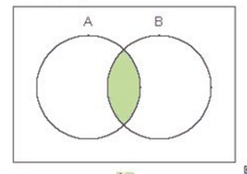
\includegraphics{D:/Dropbox/MsC UABC/2o Semestre/Clases/Estadistica/estadistica-syllabus/img/venn.png}
\caption{}
\end{figure}

\(A\cup B\)

\begin{figure}[htbp]
\centering
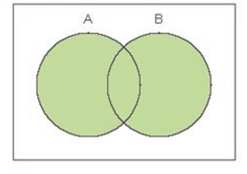
\includegraphics{D:/Dropbox/MsC UABC/2o Semestre/Clases/Estadistica/estadistica-syllabus/img/venn1.png}
\caption{}
\end{figure}

\(A^c \cap B\)

\begin{figure}[htbp]
\centering
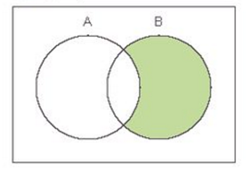
\includegraphics{D:/Dropbox/MsC UABC/2o Semestre/Clases/Estadistica/estadistica-syllabus/img/venn2.png}
\caption{}
\end{figure}

\(\text{Conjuntos Disjuntos}\)

\begin{figure}[htbp]
\centering
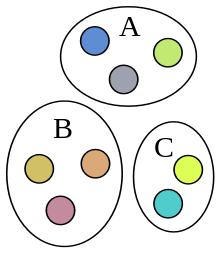
\includegraphics{D:/Dropbox/MsC UABC/2o Semestre/Clases/Estadistica/estadistica-syllabus/img/venn4.png}
\caption{}
\end{figure}

\(S,T,\space y \space V \space son \space una \space particion \space de \space \Omega\)

\begin{figure}[htbp]
\centering
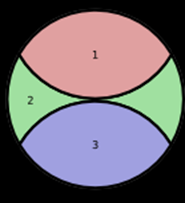
\includegraphics{D:/Dropbox/MsC UABC/2o Semestre/Clases/Estadistica/estadistica-syllabus/img/venn3.png}
\caption{}
\end{figure}

\section{Algebra de Conjuntos}\label{algebra-de-conjuntos-1}

\textbf{\emph{Propiedad asociativa ????}} \[S \cup T = T \cup S\]
\[S \cap (T \cup V) = (S \cap T) \cup (S \cap V)\] \[(S^c)^c = S\]
\[S \cup \Omega = \Omega\] \textbf{\emph{Propiedad Distributiva????}}

\[S \cup (T \cup V) = (S \cup T)\cup V\]
\[S \cup (T \cap V) = (S \cup T)\cap (S \cap V)\]
\[S \cap S^c = \emptyset\] \[S \cap \Omega = S\]

\section{Leyes de Morgan}\label{leyes-de-morgan-1}

Considerar las siguentes notaciones:
\((\bigcup_{n}^{}S_n)^c = \bigcap_{n}^{}{S_n}^c\)\\
 \((\bigcap S_n)^2 = \bigcup_{n}^{}{S_n}^c\)

*Notar como cambian de \(\cup\) a \(\cap\) y viceversa, en estas leyes.

\textbf{8 de Febrero de 2017}

\section{Modelos De Probabilidad}\label{modelos-de-probabilidad-1}

Buscan proveer certidumbre o reducir incertidumbre.

\subsection{Elementos de un Modelo de
Probabilidad}\label{elementos-de-un-modelo-de-probabilidad-1}

\begin{itemize}
\tightlist
\item
  El \textbf{espacio muestral (\(\Omega\))}: Entendido como el conjunto
  de todos los posibles resultados de un experimento.
\item
  \textbf{Ley de probabilidad}, la cual asigna a un conjunto \(A\) de
  posibles resultados (llamdo también evento) un número no-negativo
  (\(P(A) = (\text{la probabilidad de A})\)) que codifica nuestro
  conocimiento o creencia sobre la probabilidad de los elementos de
  \(A\).
\end{itemize}

\subsection{Axiomas de Probabilidad}\label{axiomas-de-probabilidad-1}

\begin{enumerate}
\def\labelenumi{\arabic{enumi}.}
\tightlist
\item
  \textbf{No negatividad} Para cada uno de los eventos en \(A\):
  \(P(A) \geq 0\)
\item
  \textbf{Adición} Si \(A\) y \(B\) son dos eventos disjuntos, entonces
  la posibilidad de su unión satisface: \(P(A \cup B) = P(A)+P(B)\)
  \textbf{ó} \(P(A_1\cup A_2 \cup ...A_n) = P(A_1) + P(A_2)+...P(A_n)\)
\item
  \textbf{Normalización} La probabilidad del copmleto (\emph{entire})
  espacio muestral \(\Omega\) es \(1\), esto es \(P(\Omega) = 1\).
\end{enumerate}

 \textbf{Ojo:} Los eventos del espacio muestral deben ser eventos
\textbf{\emph{mutuamente excluyentes}}, osea que no puedan suceder
simultaneamente.

\subsection{Ley de Probabilidad
Discreta}\label{ley-de-probabilidad-discreta-1}

\textbf{Probabilidad discreta:} Asignar a un evento una probabilidad
única (valor).

Si el espacio de probabilidad consiste de un número finito de posibles
resultados, entonces la ley de probabilidad se especifica por las
probabilidades de cada uno de los eventos. En particular, la
probabilidad de cualquier evento. \(\{S_1,S_2,...S_n\}\) es la suma de
las probabilidades de sus elementos:
\[P(\{S_1,S_2,...S_n\}) = P(S_1)+P(S_2)+...+P(S_n)\]

\subsection{Ley de Probabilidad Discreta
Uniforme}\label{ley-de-probabilidad-discreta-uniforme-1}

Si el espacio muestral consiste de \(n\) posibles resultados con igual
probabilidad de ocurrencia, entonces la probabilidad de cualquier evneto
\(A\), está dada por:
\[P(A)= \frac{\text{Número de elementos de A}}{n}\]

\subsection{\texorpdfstring{Función \emph{Densidad de
Probabilidad}}{Función Densidad de Probabilidad}}\label{funcion-densidad-de-probabilidad-1}

\begin{itemize}
\tightlist
\item
  También conocida como \emph{Probability Density Function (pdf)} o
  \emph{Probability Mass Function (pmf)}.
\end{itemize}

Para una variable aleatoria o evento discreto, se define como:
\[f(x) = P(X=x)\]

\subsection{\texorpdfstring{Acumulativa pdf (\emph{Comulative
pdf})}{Acumulativa pdf (Comulative pdf)}}\label{acumulativa-pdf-comulative-pdf-1}

\begin{itemize}
\tightlist
\item
  Se define como la suma de los resultados parcials de los eventos que
  validan el experimento:
\end{itemize}

\[cpdf = \sum_{i}(P(x_i=x))\]

Para los \(x_i\) que validan el experimento.

\textbf{14 de Febrero 2017}

\section{Probabilidad Condicional}\label{probabilidad-condicional-1}

La siguiente ecuación:

\[P(A/B) = \frac{P(A\cap B)}{P(B)}\]

Puede también ser expresada en los términos de \emph{probabilidad
condicional secuencial}: \[P(A\cap B) = P(A/B)*P(B)\] Siempre y cuando
\(P(B)>0\)

Si los posibles resultados tienen la misma probabilidad de ocurrencia
entonces:
\[P(A/B) = \frac{\text{No. de elementos en } A\cap B}{\text{No. de elementos en }B}\]

\textbf{Importante:} El conjunto universo en la probabilidad condicional
(dado un evento anterior) cambia de \(\Omega\) al subconjunto \(B\).

\subsubsection{Ejemplos:}\label{ejemplos-1}

\begin{itemize}
\tightlist
\item
  \textbf{Considerar el lanzamiento de 2 dados:}
\end{itemize}

\[A = \{\text{la suma es}\geq 8 \space y \space \leq 10\}\]
\[B = \{\text{el dado 1}=6 \} \therefore P(B) = \frac {1}{6}\]
Recordando los conceptos de combinaciones: \(C = n^m\) cuando \(n\) es
el número de posibles resultados y \(m\), el número de experimentos.
para éste ejemplo en particular las combinaciones posibles son
\(6^2 = 36\), entonces:
\[P(A\cap B) = \frac {3}{36} \therefore P(A/B) = \frac {\frac {3}{36}}{\frac {1}{6}} = \frac {18}{36} = \frac {1}{2}\]
Es importante que la probabilidad condicional es mayor a la probabilidad
independiente de previos eventos, porque el universo en la condicional
disminuye de \(\Omega\) a un subconjunto, en éste caso \(B\).

\begin{itemize}
\item
  \textbf{La probabilidad de que, al lanzar los dados del ejemplo
  anterior, la suma sea \(\geq 8\) y \(\leq 10\) ó
  \(A = \{\geq 8 \space y \space \leq 10\}.\)}

  A ésta probabilidad la denotaremos como \(P(A)\), al realizar el
  experimento manual obtenemos la siguiente imagen:

  \begin{figure}[htbp]
  \centering
  \includegraphics{D:/Dropbox/MsC UABC/2o Semestre/Clases/Estadistica/estadistica-syllabus/img/2017-02-14 11.40.56.jpg}
  \caption{}
  \end{figure}

   Se puede observar que se han indicado las combinaciones que cumplen
  con una suma \(\geq 8\) y \(\leq 10\) ó
  \(A = \{\geq 8 \space y \space \leq 10\}\).

  Por lo tanto: \[P(A) = \frac {12}{36} = \frac {1}{3}\].

  Otra manera de entender éste concepto es visualizarlo a través de una
  matriz:

  \begin{figure}[htbp]
  \centering
  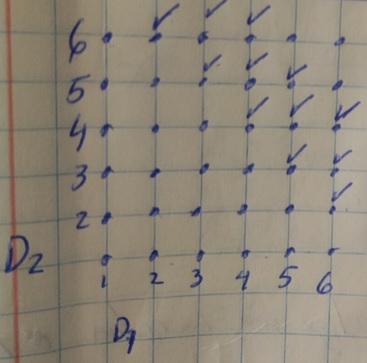
\includegraphics{D:/Dropbox/MsC UABC/2o Semestre/Clases/Estadistica/estadistica-syllabus/img/2017-02-14 12.56.55 mod.jpg}
  \caption{}
  \end{figure}
\end{itemize}

Con la visualización, es sencillo llegar a la conclusión
\(A = \frac {12}{36} = \frac {1}{3}\)

\begin{itemize}
\tightlist
\item
  \textbf{En el lanzamiento sucesivo de 3 monedas, queremos saber la
  probabilidad condicional, \(P(A/B)\), cuando \(A\) y \(B\) son los
  eventos:} \[A = \{\text{aparecen más soles que águilas}\}\]
  \[B = \{\text{el primer lanzamiento cae sol}\}\] La visualización de
  todas las posibilidades de éste fenómeno se puede apreciar en la
  siguiente figura:
\end{itemize}

\begin{figure}[htbp]
\centering
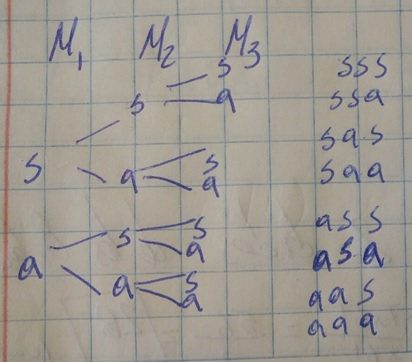
\includegraphics{D:/Dropbox/MsC UABC/2o Semestre/Clases/Estadistica/estadistica-syllabus/img/2017-02-14 12.57.08 mod.jpg}
\caption{}
\end{figure}

Derivado del árbol en la imagen se pueden determinar las probabilidades
de los siguientes subconjuntos:
\[P(A) = \{\text{sss, ssa, sas, ass }\} = \frac {4}{8} = \frac {1}{2}\]

\[P(B) = \{\text{sss, ssa, sas, saa}\} = \frac{4}{8} = \frac{1}{2}\]
\[P(A\cap B) = \{\text{sss, ssa, sas}\} = \frac{3}{8}\]

\[\therefore\]
\[P(A/B) = \frac {P(A\cap B)}{P(B)} = \frac {\frac {3}{8}}{\frac {1}{2}} = \frac {6}{8} = \frac {3}{4}\]
\textbf{\emph{Nótese el la mayor probabilidad de \(P(A/B)\) dado que el
universo pasó de ser \(\Omega\) al subconjunto \(B\).}}

\subsection{\texorpdfstring{Repaso de \textbf{combinaciones} y
\textbf{permutaciones}}{Repaso de combinaciones y permutaciones}}\label{repaso-de-combinaciones-y-permutaciones-1}

 La cantidad total de combinaciones posibles en un experimento se puede
calcular como \(n^m\) donde: \[n = \text{posibles resutlados}\]
\[m = \text{# de experimentos a realizar}\]

\begin{itemize}
\item
  Cuando de un número de combinaciones se elige una muestra \(r\) y el
  orden en el que éstas se elige no importa (\emph{combinaciones}):
  \[P = \left( \begin{array}{c} n \\ r \end{array} \right) = \frac {n!}{r!(n-r)!}\]
\item
  Cuando de un numero de combinaciones se elige una muestra \(r\) y el
  orden en el que ésta se elige \textbf{SI} importa
  (\emph{permutaciones}):
  \[P = \left( \begin{array}{c} n \\ r \end{array} \right) = \frac {n!}{(n-r)!}\]
\end{itemize}

\subsubsection{Ejemplo:}\label{ejemplo-2}

Al lanzar 8 dados, ¿cuántas combinaciones diferentes son posibles?
\[C = 6^8\] \textbf{PENDIENTE REVISAR}- Si elijo el resultado de 2 dados
de los 8 lanzados, ¿de cuántas maneras distintas los puedo elegir?:

\[P = \left( \begin{array}{c} 8 \\ 2 \end{array} \right) = \frac {n!}{r!(n-r)!}\]

Siempre y cuando \(A_1\) y \(A_2\) sean eventos disjuntos
(\(P(A_1\cap A_2) = \emptyset\)) podemos entonces decir que:

\[P = (A_1 \cap A_2 \vert B) = \frac {P(A_1 \cap B)}{P(B)}+ \frac {P(A_2 \cap B)}{P(B)} = P(A_1/B) + P(A_2/B)\]

\subsubsection{Ejemplo}\label{ejemplo-3}

Tomando datos del experimento anterior con monedas:

\[A_1 = \{\text{aparecen más soles que águilas}\} = \{\text{sss, ssa, sas, ass}\}\]
\[A_2 = \{\text{aparecen más águilas que soles}\} = \{\text{ssa, asa, aas, aaa}\}\]
\[B = \{\text{el primer lanzamiento es sol}\} = \{\text{sss, ssa, sas, saa}\}\]
\[A_1 \cap A_2 = \{\emptyset\}\] \[\therefore\]
\[P(A_1) = \frac {4}{8} = \frac {1}{4}\space \& \space P(A_2) = \frac {4}{8} = \frac {1}{4}\]
\[P(A_1\cap B) = \frac{3}{8}\] \[P(A_2\cap B) = \frac{1}{8}\]
\[P(A_1\cup A_2\vert B) = \frac {\frac{3}{8}}{\frac{1}{2}} + \frac{\frac{1}{8}}{\frac{1}{2}} = \frac{6}{8} + \frac{2}{8} = 1\]
\[P(A_1\cup A_2\vert B) = 1 \space \therefore\]
\[P(A_1\cup A_2...\cup A_i \vert B) = P(A_1/B) + P(A_2/B)+...+ P(A_i/B)\]
Siempre y cuando \(\{A_1\cap A_2...\cap A_i\}= \emptyset\).

\subsection{Independencia}\label{independencia-1}

Si: \[P(A\cap B) = P(A)*P(B)\] Se dice que \(A\) y \(B\) son eventos
\textbf{independientes}. Distinto a ser eventos disjuntos:
\(P(A\cap B) = \emptyset\). Entonces, asumiendo independencia obetnemos:

\[P(A/B) = \frac {P(A\cap B)}{P(B)} = \frac{P(A)P(B)}{P(B)} = P(A)\]

La ecuación anterior demuestra que, los eventos independientes no
afectan la probabilidad uno del otro.

\chapter{Literature}\label{literature}

\chapter{Methods}\label{methods-1}

\chapter{Applications}\label{applications-1}

\chapter{Final Words}\label{final-words-1}

\chapter{Placeholder}\label{placeholder}

\bibliography{packages,book}


\end{document}
